\documentclass[12pt,a4paper]{article}

\usepackage[margin=1.5cm]{geometry}
\usepackage{amsmath,amssymb}
\usepackage{tikz}
\usetikzlibrary{arrows.meta}

\setlength{\parindent}{0pt}
\pagestyle{empty}

% ---------- TikZ axes (used in the templates) ----------
\newcommand{\ParabolaAxes}{
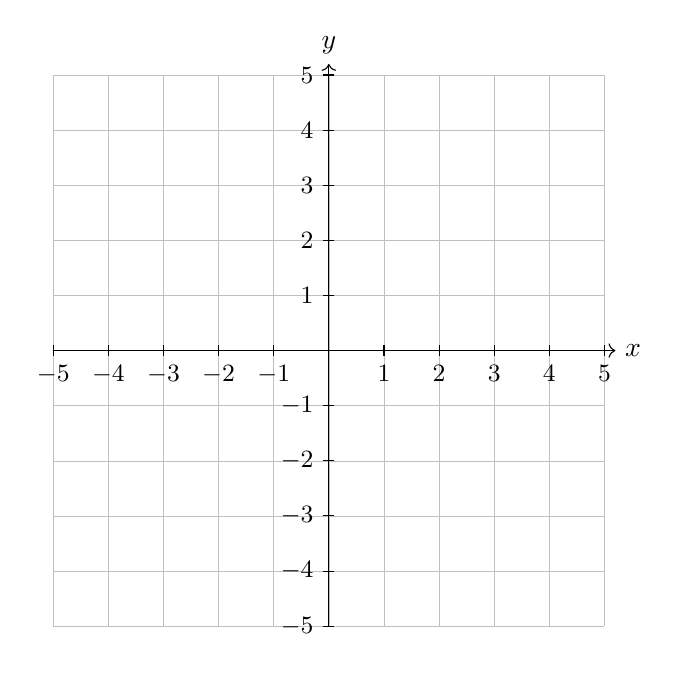
\begin{tikzpicture}[scale=0.7]
  % Grid
  \draw[step=1cm,very thin,gray!50] (-5,-5) grid (5,5);
  % Axes
  \draw[->] (-5,0) -- (5.2,0) node[right] {$x$};
  \draw[->] (0,-5) -- (0,5.2) node[above] {$y$};
  % Ticks on x-axis
  \foreach \x in {-5,-4,...,5} {
    \draw (\x,0.1) -- (\x,-0.1);
    \ifnum\x=0\else
      \node[below=2pt] at (\x,0) {\small $\x$};
    \fi
  }
  % Ticks on y-axis
  \foreach \y in {-5,-4,...,5} {
    \draw (0.1,\y) -- (-0.1,\y);
    \ifnum\y=0\else
      \node[left=2pt] at (0,\y) {\small $\y$};
    \fi
  }
\end{tikzpicture}
}

% ---------- TEMPLATE: Standard form ----------
\newcommand{\StandardParabolaTemplate}{
\noindent
\fbox{%
\begin{minipage}[t]{0.46\textwidth}
\textbf{Equation:} \rule{0.9\linewidth}{0.4pt}

\vspace{0.3cm}
\textbf{Identify the coefficients}\\[1ex]
$a = \rule{1.2cm}{0.4pt} \quad
 b = \rule{1.2cm}{0.4pt} \quad
 c = \rule{1.2cm}{0.4pt}$

\vspace{0.4cm}
\textbf{1. General shape}\\[0.5ex]
Circle one: \quad \textbf{happy} / \textbf{sad}\\[0.5ex]
Reason: $a$ is \rule{2.5cm}{0.4pt}
(positive/negative).

\vspace{0.4cm}
\textbf{2. $y$-intercept}\\[0.5ex]
Substitute $x = 0$ into $y = ax^2 + bx + c$:\\[0.5ex]
$y = a(0)^2 + b(0) + c = \rule{2.5cm}{0.4pt}$\\[0.5ex]
Point: $(0,\rule{2cm}{0.4pt})$

\vspace{0.4cm}
\textbf{3. $x$-intercepts}\\[0.5ex]
Solve $ax^2 + bx + c = 0$\\
(using factorising or the quadratic formula).\\[0.5ex]
$x_1 = \rule{2.5cm}{0.4pt}$\\[0.5ex]
$x_2 = \rule{2.5cm}{0.4pt}$

\vspace{0.4cm}
\textbf{4. Turning point}\\[0.5ex]
Use $x = -\dfrac{b}{2a}$:\\[0.5ex]
$x_{\text{TP}} = -\dfrac{b}{2a} = \rule{2.5cm}{0.4pt}$\\[0.5ex]
Substitute this $x$ into the equation to find $y$:\\[0.5ex]
$y_{\text{TP}} = \rule{2.5cm}{0.4pt}$\\[0.8ex]
Turning point: $\big(\rule{1.8cm}{0.4pt},\rule{1.8cm}{0.4pt}\big)$
\end{minipage}
\hspace{0.02\textwidth}
\begin{minipage}[t]{0.48\textwidth}
\centering
\ParabolaAxes
\end{minipage}
} % end fbox
\vspace{0.5cm}
}

% ---------- TEMPLATE: Turning-point form ----------
\newcommand{\TurningPointParabolaTemplate}{
\noindent
\fbox{%
\begin{minipage}[t]{0.46\textwidth}
\textbf{Equation:} \rule{0.9\linewidth}{0.4pt}

\vspace{0.3cm}
\textbf{Identify the parameters}\\[1ex]
$a = \rule{1.2cm}{0.4pt} \quad
 h = \rule{1.2cm}{0.4pt} \quad
 k = \rule{1.2cm}{0.4pt}$

\vspace{0.4cm}
\textbf{1. General shape}\\[0.5ex]
Circle one: \quad \textbf{happy} / \textbf{sad}\\[0.5ex]
Reason: $a$ is \rule{2.5cm}{0.4pt}
(positive/negative).

\vspace{0.4cm}
\textbf{2. Turning point}\\[0.5ex]
From $y = a(x-h)^2 + k$, the turning point is:\\[0.5ex]
$(h,k) = \big(\rule{1.8cm}{0.4pt},\rule{1.8cm}{0.4pt}\big)$

\vspace{0.4cm}
\textbf{3. $y$-intercept}\\[0.5ex]
Substitute $x = 0$:\\[0.5ex]
$y = a(0-h)^2 + k = \rule{2.5cm}{0.4pt}$\\[0.5ex]
Point: $(0,\rule{2cm}{0.4pt})$

\vspace{0.4cm}
\textbf{4. $x$-intercepts}\\[0.5ex]
Solve $a(x-h)^2 + k = 0$\\[0.5ex]
$(x-h)^2 = \rule{2.5cm}{0.4pt}$\\[0.5ex]
$x_1 = \rule{2.5cm}{0.4pt}$\\[0.5ex]
$x_2 = \rule{2.5cm}{0.4pt}$

\end{minipage}
\hspace{0.02\textwidth}
\begin{minipage}[t]{0.48\textwidth}
\centering
\ParabolaAxes
\end{minipage}
} % end fbox
\vspace{0.5cm}
}

\begin{document}

% =====================================================
%  INSTRUCTION SHEET 1: STANDARD FORM
% =====================================================
\begin{center}
  {\LARGE Sketching Parabolas from Standard Form}\\[0.5cm]
  \textbf{Parabolas of the form} \quad $y = ax^2 + bx + c$
\end{center}

\textbf{Goal:} Sketch the parabola and clearly show the \emph{general shape} (happy/sad), the \emph{$y$-intercept}, the \emph{$x$-intercepts}, and the \emph{turning point}.

\vspace{0.3cm}

\textbf{Step 1: Identify $a$, $b$, and $c$.}\\[0.3ex]
Write the equation in the form $y = ax^2 + bx + c$ and read off:
\[
a = \_\_\_\_, \quad b = \_\_\_\_, \quad c = \_\_\_\_.
\]

\textbf{Step 2: General shape (happy or sad).}\\[0.3ex]
\begin{itemize}
  \item If $a > 0$, the parabola opens upwards. You can describe it as \textbf{happy} (concave up).
  \item If $a < 0$, the parabola opens downwards. You can describe it as \textbf{sad} (concave down).
\end{itemize}

\textbf{Step 3: $y$-intercept.}\\[0.3ex]
The $y$-intercept is where the graph crosses the $y$-axis. Here, $x = 0$.
\[
y = a(0)^2 + b(0) + c = c.
\]
So the $y$-intercept is the point $(0,c)$.

\textbf{Step 4: $x$-intercepts.}\\[0.3ex]
The $x$-intercepts are where the graph crosses the $x$-axis. Here, $y = 0$.
\[
0 = ax^2 + bx + c.
\]
\begin{itemize}
  \item Try \textbf{factorising} if possible.
  \item If it will not factorise nicely, use the \textbf{quadratic formula}:
  \[
  x = \frac{-b \pm \sqrt{b^2 - 4ac}}{2a}.
  \]
\end{itemize}
You may get:
\begin{itemize}
  \item Two $x$-intercepts (two real solutions),
  \item One $x$-intercept (a repeated root, the parabola just touches the $x$-axis), or
  \item No real $x$-intercepts (the parabola does not cross the $x$-axis).
\end{itemize}

\textbf{Step 5: Turning point.}\\[0.3ex]
The turning point is the highest or lowest point on the parabola.
\begin{itemize}
  \item The $x$-coordinate of the turning point is
  \[
  x_{\text{TP}} = -\frac{b}{2a}.
  \]
  \item Substitute this into the equation to find the $y$-coordinate:
  \[
  y_{\text{TP}} = a\left(-\frac{b}{2a}\right)^2
                  + b\left(-\frac{b}{2a}\right)
                  + c.
  \]
\end{itemize}
So the turning point is
\[
\big(x_{\text{TP}}, y_{\text{TP}}\big)
=
\left(-\frac{b}{2a},\; f\!\left(-\frac{b}{2a}\right)\right).
\]

\textbf{Step 6: Sketching the parabola.}\\[0.3ex]
\begin{itemize}
  \item Plot the $y$-intercept.
  \item Plot any $x$-intercepts you found.
  \item Plot the turning point.
  \item Use the general shape (happy/sad) and symmetry about the vertical line $x = x_{\text{TP}}$ to sketch a smooth curve.
\end{itemize}

\vspace{0.6cm}
\textbf{Worked example A (happy parabola).}\\[0.4ex]
Sketch $y = x^2 - 4x + 3$.

\begin{enumerate}
  \item Identify $a$, $b$, $c$:
  \[
  a = 1,\quad b = -4,\quad c = 3.
  \]
  \item Shape:
  \[
  a = 1 > 0 \Rightarrow \text{parabola is \textbf{happy} (opens up).}
  \]
  \item $y$-intercept:
  \[
  y = c = 3 \Rightarrow (0,3).
  \]
  \item $x$-intercepts: solve $x^2 - 4x + 3 = 0$.
  \[
  x^2 - 4x + 3 = (x-1)(x-3) = 0
  \Rightarrow x = 1 \text{ or } x = 3.
  \]
  So the $x$-intercepts are $(1,0)$ and $(3,0)$.
  \item Turning point:
  \[
  x_{\text{TP}} = -\frac{b}{2a} = -\frac{-4}{2 \cdot 1} = 2.
  \]
  Substitute $x = 2$:
  \[
  y_{\text{TP}} = 2^2 - 4\cdot 2 + 3 = 4 - 8 + 3 = -1.
  \]
  Turning point is $(2,-1)$.
  \item Sketch using the points $(0,3)$, $(1,0)$, $(2,-1)$, $(3,0)$ and a happy shape.
\end{enumerate}

\vspace{0.4cm}
\textbf{Worked example B (sad parabola).}\\[0.4ex]
Sketch $y = -x^2 - 2x + 3$.

\begin{enumerate}
  \item Identify $a$, $b$, $c$:
  \[
  a = -1,\quad b = -2,\quad c = 3.
  \]
  \item Shape:
  \[
  a = -1 < 0 \Rightarrow \text{parabola is \textbf{sad} (opens down).}
  \]
  \item $y$-intercept:
  \[
  y = c = 3 \Rightarrow (0,3).
  \]
  \item $x$-intercepts: solve $-x^2 - 2x + 3 = 0$.
  \[
  -x^2 - 2x + 3 = 0
  \Rightarrow x^2 + 2x - 3 = 0
  \Rightarrow (x+3)(x-1) = 0.
  \]
  So $x = -3$ or $x = 1$, giving $(-3,0)$ and $(1,0)$.
  \item Turning point:
  \[
  x_{\text{TP}} = -\frac{b}{2a}
  = -\frac{-2}{2\cdot(-1)} = \frac{2}{-2} = -1.
  \]
  Substitute $x = -1$:
  \[
  y_{\text{TP}} = -(-1)^2 - 2(-1) + 3 = -1 + 2 + 3 = 4.
  \]
  Turning point is $(-1,4)$.
  \item Sketch using $(0,3)$, $(-3,0)$, $(1,0)$, $(-1,4)$ and a sad shape.
\end{enumerate}

\newpage

% =====================================================
%  INSTRUCTION SHEET 2: TURNING-POINT FORM
% =====================================================
\begin{center}
  {\LARGE Sketching Parabolas from Turning-Point Form}\\[0.5cm]
  \textbf{Parabolas of the form} \quad $y = a(x-h)^2 + k$
\end{center}

\textbf{Goal:} Sketch the parabola and clearly show the \emph{general shape} (happy/sad), the \emph{turning point}, the \emph{$y$-intercept}, and the \emph{$x$-intercepts}.

\vspace{0.3cm}

\textbf{Step 1: Identify $a$, $h$, and $k$.}\\[0.3ex]
Write the equation in the form $y = a(x-h)^2 + k$ and read off:
\[
a = \_\_\_\_, \quad h = \_\_\_\_, \quad k = \_\_\_\_.
\]

\textbf{Step 2: General shape (happy or sad).}\\[0.3ex]
\begin{itemize}
  \item If $a > 0$, the parabola opens upwards (\textbf{happy}).
  \item If $a < 0$, the parabola opens downwards (\textbf{sad}).
\end{itemize}

\textbf{Step 3: Turning point.}\\[0.3ex]
From $y = a(x-h)^2 + k$:
\begin{itemize}
  \item The turning point is directly given as $(h,k)$.
  \item The axis of symmetry is the vertical line $x = h$.
\end{itemize}

\textbf{Step 4: $y$-intercept.}\\[0.3ex]
Set $x = 0$ and substitute into the equation:
\[
y = a(0-h)^2 + k.
\]
This gives the $y$-intercept at the point $(0,y)$.

\textbf{Step 5: $x$-intercepts.}\\[0.3ex]
Set $y = 0$ and solve
\[
0 = a(x-h)^2 + k.
\]
\begin{itemize}
  \item Rearrange to isolate $(x-h)^2$.
  \item Take square roots to find $x-h$.
  \item Solve for $x$ to get one or two $x$-intercepts (or none, if there are no real solutions).
\end{itemize}

\textbf{Step 6: Sketching the parabola.}\\[0.3ex]
\begin{itemize}
  \item Plot the turning point $(h,k)$.
  \item Plot the $y$-intercept.
  \item Plot any $x$-intercepts found.
  \item Use the general shape (happy/sad) and the symmetry about $x = h$ to draw a smooth curve.
\end{itemize}

\vspace{0.6cm}
\textbf{Worked example C (happy parabola).}\\[0.4ex]
Sketch $y = 2(x-1)^2 - 3$.

\begin{enumerate}
  \item Identify $a$, $h$, $k$:
  \[
  a = 2,\quad h = 1,\quad k = -3.
  \]
  \item Shape:
  \[
  a = 2 > 0 \Rightarrow \text{parabola is \textbf{happy} (opens up).}
  \]
  \item Turning point:
  \[
  (h,k) = (1,-3).
  \]
  \item $y$-intercept: set $x = 0$.
  \[
  y = 2(0-1)^2 - 3 = 2(1) - 3 = -1.
  \]
  So the $y$-intercept is $(0,-1)$.
  \item $x$-intercepts: set $y = 0$.
  \[
  0 = 2(x-1)^2 - 3
  \Rightarrow 2(x-1)^2 = 3
  \Rightarrow (x-1)^2 = \frac{3}{2}.
  \]
  Take square roots:
  \[
  x - 1 = \pm\sqrt{\frac{3}{2}}
  \Rightarrow x = 1 \pm \sqrt{\frac{3}{2}}.
  \]
  (You can leave these as exact surds.)
  \item Sketch using the turning point $(1,-3)$, the $y$-intercept $(0,-1)$ and symmetric $x$-intercepts.
\end{enumerate}

\vspace{0.4cm}
\textbf{Worked example D (sad parabola).}\\[0.4ex]
Sketch $y = -\dfrac{1}{2}(x+2)^2 + 4$.

\begin{enumerate}
  \item Identify $a$, $h$, $k$:
  \[
  a = -\frac{1}{2},\quad h = -2,\quad k = 4.
  \]
  (Because $x+2 = x - (-2)$.)
  \item Shape:
  \[
  a = -\frac{1}{2} < 0 \Rightarrow \text{parabola is \textbf{sad} (opens down).}
  \]
  \item Turning point:
  \[
  (h,k) = (-2,4).
  \]
  \item $y$-intercept: set $x = 0$.
  \[
  y = -\frac{1}{2}(0+2)^2 + 4
    = -\frac{1}{2}\cdot 4 + 4
    = -2 + 4
    = 2.
  \]
  So the $y$-intercept is $(0,2)$.
  \item $x$-intercepts: set $y = 0$.
  \[
  0 = -\frac{1}{2}(x+2)^2 + 4
  \Rightarrow -\frac{1}{2}(x+2)^2 = -4
  \Rightarrow (x+2)^2 = 8.
  \]
  Take square roots:
  \[
  x + 2 = \pm\sqrt{8} = \pm 2\sqrt{2}
  \Rightarrow x = -2 \pm 2\sqrt{2}.
  \]
  \item Sketch using turning point $(-2,4)$, $y$-intercept $(0,2)$ and the two $x$-intercepts $(-2\pm 2\sqrt{2},0)$.
\end{enumerate}

\newpage

% =====================================================
%  BLANK TEMPLATES: STANDARD FORM
% =====================================================
\begin{center}
  {\LARGE Parabola Sketching Template}\\[0.2cm]
  \textbf{Standard Form:} $y = ax^2 + bx + c$
\end{center}

\StandardParabolaTemplate

\StandardParabolaTemplate

\newpage

% =====================================================
%  BLANK TEMPLATES: TURNING-POINT FORM
% =====================================================
\begin{center}
  {\LARGE Parabola Sketching Template}\\[0.2cm]
  \textbf{Turning-Point Form:} $y = a(x-h)^2 + k$
\end{center}

\TurningPointParabolaTemplate

\TurningPointParabolaTemplate

\end{document}
